% vim: set tw=78 sts=2 sw=2 ts=8 aw et ai:

Tests were run for low and high bandwidths, starting from 1 Mbps and doubling up to 1024 Mbps (which actually had to be 1000 Mbps because of Mininet limitations). In figures \ref{fig:16mbps-cw} and \ref{fig:16mbps-d}  we can observe the influence of two major parameters on the throughput for an average value of 16 Mbps for the bandwidth of one link and no loss on either channel. The setup is the one that was described in the previous section.

\begin{figure}
  \centering
  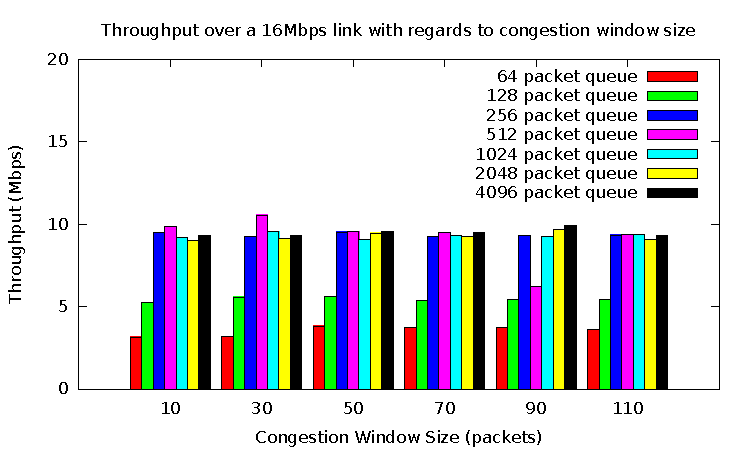
\includegraphics[width=0.85\textwidth]{img/throughput-cwnd-16Mbps}
  \caption{Congestion window impact}
  \label{fig:16mbps-cw}
\end{figure}

\begin{figure}
  \centering
  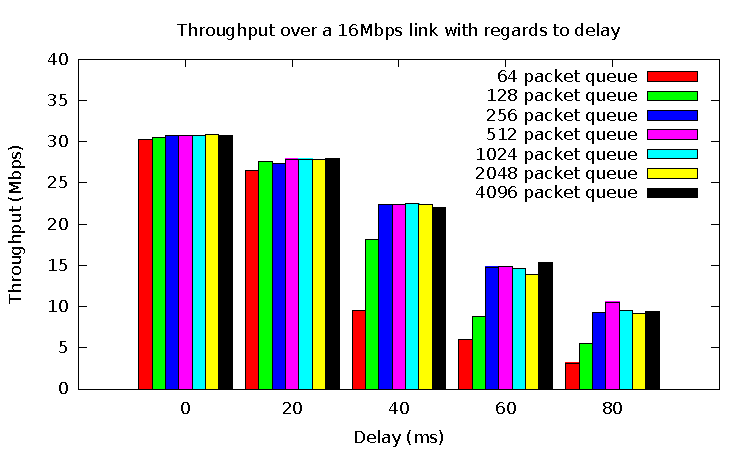
\includegraphics[width=0.85\textwidth]{img/throughput-delay-16Mbps}
  \caption{Channel delay impact}
  \label{fig:16mbps-d}
\end{figure}

Figure \ref{fig:16mbps-cw} shows the impact of the congestion window's initial size correlated with the receiving queue size. The channel has no losses and the link delay is 80 seconds. It is noticeable that the initial size of the congestion window does not affect performance too much because MPTCP's algorithm is adapting it over the course of the data transfer. Throughput is better for larger receive buffers, but it reaches a ceiling of approximately 10 Mbps because of the sizeable delay.

Figure \ref{fig:16mbps-d} outlines the impact of delay. MPTCP's performance is close to the maximum possible throughput of 32 Mbps regardless of the receive buffer when there is zeo delay. The performance expectedly decreases when delay is larger and we notice that the receive buffer size starts to influence throughput. That is because the size of the receive buffer is conditioned by the bandwidth-delay product as it was mentioned in \ref{sec:related}.

\begin{figure}
  \centering
  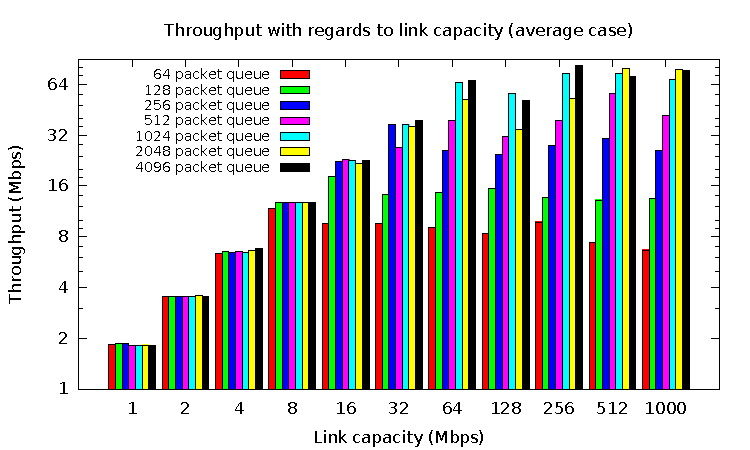
\includegraphics[width=\textwidth]{img/throughput-bdw-avg}
  \caption{Link capacity impact with average delay}
  \label{fig:bdw-avg}
\end{figure}

\begin{figure}
  \centering
  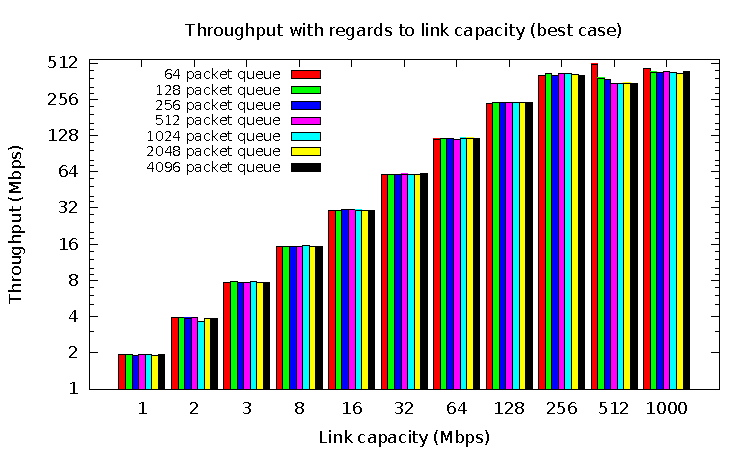
\includegraphics[width=\textwidth]{img/throughput-bdw-max}
  \caption{Link capacity impact with no delay}
  \label{fig:bdw-max}
\end{figure}

\begin{figure}
  \centering
  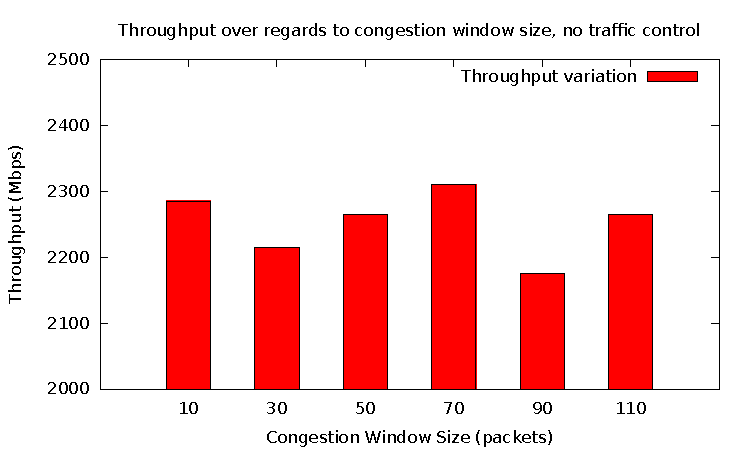
\includegraphics[width=0.85\textwidth]{img/throughput-cwnd-notc}
  \caption{Throughput without overhead associated with traffic control}
  \label{fig:cwnd-notc}
\end{figure}

